\chapter{Fazit} \label{sec:conclusion}

In diesem abschließenden Kapitel werden zunächst die implementierten Verfahren anhand ihrer Testergebnisse und Eigenschaften für den möglichen Einsatz in Augmented Reality Anwendungen eingeschätzt. Dazu werden die Ergebnisse aus den statischen Testszenen als auch die Einschätzungen in der dynamisch getesteten Anwendung in die Ergebnisse einfließen. Hiernach soll zudem noch ein Ausblick gegeben werden, wie eine potentielle Weiterentwicklung der Verfahren aussehen könnte und welche technischen Änderungen in Project Tango einen verbesserten Einsatz der Verfahren begünstigen würden.

\section{Evaluation}

Die prototypische Umsetzung der Verfahren zeigt, dass mit dem grundlegenden Ansatz der Tiefenbild Überdeckung von \citet{wloka1995resolving} eine Echtzeit Überdeckung virtueller Objekte auch auf der mobilen Project Tango Hardware erfolgreich umgesetzt werden kann. Dabei wird im Folgenden auf jedes Verfahren sowie ihrer Vor und Nachteile im Kontext der anderen Verfahren und auf Basis der durchgeführten Tests eingegangen. 

\subsection*{Pointcloud Projektion}

Die Überlagerung durch die Pointcloud Projektion bietet gegenüber den anderen Verfahren den Vorteil, dass sie zu jeder Zeit eine dynamische und aktualisierte Repräsentation der Tiefe von der Szene liefert und somit auch Änderungen in der Szene sofort berücksichtigt. Außerdem ist das Verfahren nicht auf Clustergrößen beschränkt und kann dadurch auch komplexe Strukturen abbilden. Zu erkennen ist das in der Testszene zwei, bei der die Bilddifferenz zum optimalen Ergebnis am geringsten ist, obwohl die Pflanze eine komplexe Struktur besitzt, an denen die anderen Verfahren scheitern.

Dadurch, dass die Pointcloud von Project Tango Fehler in Form von Ausreißern und einem gewissem Rauschen enthalten kann, spiegeln sich diese Fehler auch in der berechneten Projektion wieder. Das führt dazu, dass zum Beispiel die Kante einer realen Überlagerung durchgehend in Bewegung ist und Ihre Struktur mit jedem neuen Tiefenbild variiert. Ein weiteres Problem dieser Technik ist, dass sie, dadurch dass sie sich nur auf einen Datensatz pro Aufnahme bezieht, die Tiefe nur innerhalb des Messbereichs des Tiefensensors repräsentieren kann. Dadurch können Überlagerungen von realen Objekten innerhalb der ersten 50 Zentimeter und ab vier Metern nicht mehr bestimmt werden. Durch das Zeichnen der Tiefe mit den Punkt Primitiven eines bestimmten Radius entstehen zusätzliche Fehler, denn die Abbildung von, zum Beispiel, schräg angesiedelte Flächen enthalten sichtbare Quantisierungsstufen.

\subsection*{Ebenen Rekonstruktion}

Die Ebenen Rekonstruktion löst die Schwächen der Pointcloud Projektion in dem Sinne, dass sie die Ungenauigkeit der Tiefeninformation als eine Oberflächen Approximation mit Hilfe von RANSAC in Form von Ebenen abbildet. Hierdurch werden Ausreißer weitestgehend ignoriert und auch das Rauschen bezüglich der Oberfläche wird durch eine lineare Regression gemittelt. Zusätzlich ermöglicht das Vorgehen der Ebenen Rekonstruktion eine kontinuierliche Verbesserung, indem alle bereits aufgenommenen Pointclouds in die aktuelle Rekonstruktion einfließen. Auch wenn dieser Rekonstruktionsansatz durch den Octree eine Rekonstruktion in einer groben Struktur, den Clustern des Octrees, durchführt, erhält das Verfahren durch das Ermitteln der konvexen Hülle pro gefundener Ebene einen gewissen Detailgrad, um auch schwierige planare Strukturen abbilden zu können. Die gemessenen Ergebnisse der Szenen eins und zwei spiegeln diese positive Eigenschaft wieder und zeigen, dass diese Art der Rekonstruktion auch komplexe Szenen für dieses Testszenario gut abbilden kann.

In einem manuellen dynamischeren Test mit Bewegungen weißt dieses Verfahren jedoch einige Schwächen auf. So sind durch die begrenzte Dichte der Pointcloud Lücken zwischen den Ebenen zu sehen, die zwar von Aufnahme zu Aufnahme kleiner werden aber üblicherweise nicht komplett schließen. Das führt dazu, dass zum Beispiel große Oberflächen, die ein virtuelles Objekt überlagern, das Objekt vereinzelt nicht aussparen, da keine Tiefe an den Stellen durch Lücken zwischen den Ebenen vorhanden ist. Außerdem ist das Verfahren nur bedingt in der Lage runde Strukturen wie den Sitzball aus Szene eins zu rekonstruieren. Diese Fehler werden besonders dann sichtbar, wenn man sich um diesen Ball dreht und er eine Überlagerung mit den Ecken und Kanten der Ebenen aus der Rekonstruktion auf ein virtuelles Objekt ausübt. Neben der fehlenden Unterstützung für runde Konturen besitzt dieses Verfahren keine Möglichkeit, Messungen zu revidieren wenn reale Objekte in der Szene verändert wurden oder ein Drift Fehler von Project Tango auftritt.

\subsection*{TSDF Rekonstruktion}

Wie zu erwarten liefert Chisel als eine TSDF Implementierung, aufgrund der großen Voxelgröße, nicht die Qualität, die zum Beispiel ein KinectFusion liefern kann. Dafür ist es performant genug, um als eine CPU Implementierung eine Echtzeit Rekonstruktion auf der mobilen Project Tango Hardware zu ermöglichen. Genau wie die Ebenen Rekonstruktion bietet Chisel den Vorteil eine Rekonstruktion pro Tiefenbild anzureichern und stetig zu verbessern. Dadurch können Überlagerungen auch außerhalb des Messbereichs des Tiefensensors ermöglicht werden. Anders als bei der Ebenen Rekonstruktion generiert die TSDF Rekonstruktion stets eine geschlossene Oberfläche. Außerdem können runde Strukturen festgehalten werden, wodurch der in Szene eins stehende Sitzball abgebildet werden kann.

Die große Voxelgöße führt jedoch dazu, dass wie in beiden getesteten Szenen zu erkennen, die Strukturen der Rekonstruktionen sehr grob ausfallen und dadurch die Differenzergebnisse ohne eine Filterung auf einen hohen Fehler hinweisen. Auch wenn Chisel nicht in der Lage ist die detaillierten Kantenabbildungen wie die Ebenen Rekonstruktion zu generieren, besitzt Chisel einen Vorteil: Durch den Space Carving Mechanismus können Rekonstruktionen wieder revidiert werden. Das hilft dabei den Problematiken des Drift Effekts von Project Tango entgegenzuwirken. Außerdem könnte dieses Rekonstruktionsverfahren durch eine GPU Implementierung mit deutlich kleinerer Voxelgröße und dadurch höherem Detailgrad realisiert werden.

\subsection*{Guided Filter}

Der Guided Filter war in den Tests häufig in der Lage selbst grobe Fehler im Tiefenbild an die Kanten der Farbbilder anzugleichen und somit auch, wie in den Messergebnissen zu erkennen, den Differenzwert zum Optimum zu reduzieren. Jedoch führte der Einsatz des Filters zu deutlichen Performanceeinbußen, denn der Filterprozess selbst benötigt im Durchschnitt \(220\) ms. Der Einsatz von OpenCV erschwert zudem den Einsatz des Filters für die Echtzeit Umsetzung, da die Bildebene pro Bild aus dem OpenGL Framebuffer heraus und wieder hinein geladen werden muss. Dieser Prozess benötigt zusätzliche \(80\) ms, was die Wiederholrate der prototypischen Implementierung auf 3 Herz reduziert. 

Zusätzlich sind unter gewissen Umständen, bei denen ein virtuelles Objekt nah an der Oberfläche eines realen Objekts, aber immer noch räumlich hinter dem realen Objekt liegt, Artefakte aufgefallen, an denen das eigentlich überlagerte virtuelle Objekt durchschimmert. Dieser Effekt ist in Abbildung \ref{fig:artifacts} zu erkennen. Denn neben den eigentlichen Kanten für die Überlagerung im Farbbild werden auch Kanten von flachen Strukturen berücksichtigt. Im Bild zu sehen, beeinflusst das Muster vom Würfel das resultierende Tiefenbild soweit, dass eine fehlerhafte Überlagerung nach der Filterung stattfindet. Zudem ist zu beachten, dass das Tiefenbild durch die Konvertierung von \(16\) zu \(8\) Bit Zwischenschritte verliert, wodurch dieser Effekt begünstigt wird. So liegt bei \(16\) Bit die Auflösung der Tiefe mit einer hinteren Clippingebene von \(10 m\) noch bei \(0.0152 cm\), wo bei einer \(8\) Bit Kodierung diese nur noch bei \(3.90 cm\) liegt.
 
\begin{figure}[h]
  \centering
	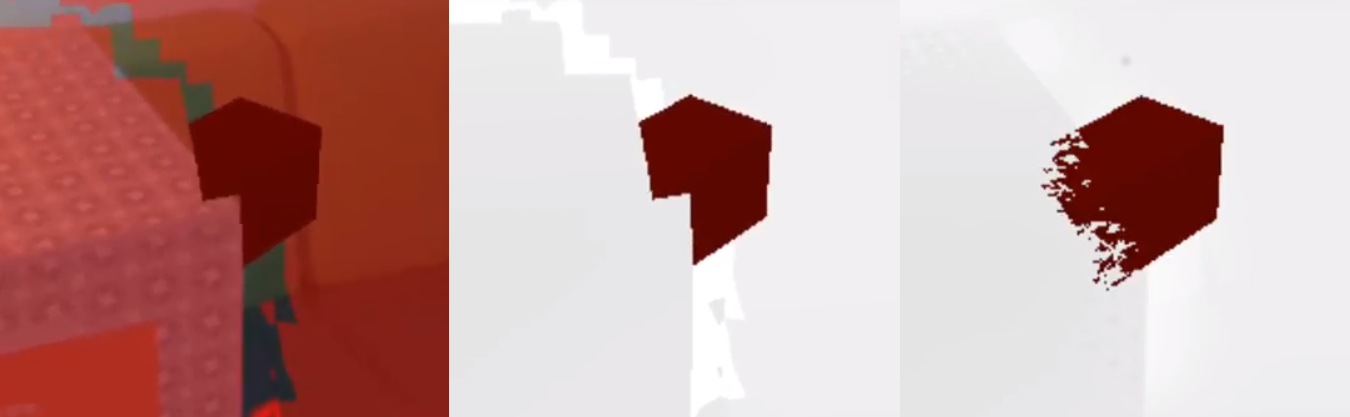
\includegraphics[width=1.0\textwidth]{content/images/artifacts.png} 
  \caption{Fehlerhafte Überdeckung bei der Anwendung des Guided Filters. Links: Reales Objekt mit Rekonstruktion. Mitte: Tiefenbild. Rechts: Sichtbare Fehler nach Guided Filter.}
  \label{fig:artifacts}
\end{figure}

Angewendet auf die Tiefeninformationen der Pointcloud Projektion konnte der Filter in der komplexeren zweiten Szene nahezu das Optimum der Überlagerung erreichen. Schwieriger war jedoch der Einsatz bei der runden Kontur in der ersten Szene, wo der Filter nicht in der Lage war, den initialen groben Fehler vom Tiefensensor zu revidieren. Das selbe Verhalten ist auch bei der Ebenen Rekonstruktion in Szene eins zu beobachten. 

Besonders beachtenswert ist die Tatsache, dass bei den zu weit reichenden Tiefeninformationen der TSDF Rekonstruktion, in der Mitte der Messergebnisse von Szene eins, ein etwa gleichgroßer Fehler durch die Filterung behoben werden konnte. Eine weitere Besonderheit, die während der Tests zu erkennen war, ist dass der Filter in der Lage war bei der Anwendung auf die Tiefeninformationenen der Ebenen Rekonstruktion, die Lücken zwischen den Ebenen unkenntlich zu machen. Somit würde dieser Filter einen Nachteil der Ebenen Rekonstruktion lösen.

\section{Einsatz der Verfahren}

Grundsätzlich ist festzuhalten, dass sich die Pointcloud Projektion ohne den Guided Filter, trotz des erreichbaren Detailgrads, höchstens in einzelnen Bildaufnahmen für eine Überlagerung in Augmented Reality eignet, da das Rauschen der Eingangsdaten durchgehend sichtbar ist. Außerdem ist die Sichtweite auf die Erreichbarkeit des Tiefensensors des aktuellen Ausschnitts begrenzt. Auch die Ebenen Rekonstruktion ist ohne Filterung bedingt geeignet, da Lücken zwischen den Ebenen zu erkennen sind, die die Illusion von AR zerstören würde. Auch wenn die TSDF Rekonstruktionen durch Chisel nach den statischen Testszenen oft mit Fehler behaftet waren, existieren entschiedene Vorteile gegenüber den anderen Vorgehensweisen. Denn durch Chisel werden geschlossene Flächen gebildet, welche sich dynamisch der Szene anpassen können. Betrachtet man zudem den Einsatz von Chisel in größeren Flächen, wie in Räumen oder sogar im ganzen Gebäude, fällt der gemessene Fehler deutlich weniger auf.\\

Angenommen, man würde den Guided Filters im Prototypen für jedes Verfahren in Echtzeit anwenden können, so würde die Pointcloud Projektion durchaus Anwendung finden. Es könnte zum Beispiel in einer AR Applikation genutzt werden, die sich nur in einem bestimmten Sichtbereich bewegt, und die eine gewisse komplexe und dynamische Szene bedienen muss. Ausgehend von den Testergebnissen als Entscheidung zwischen der Ebenen Rekonstruktion und der TSDF Rekonstruktion mit dem Guided Filter würde, wie auch ohne Filter, Chisel die bessere Alternative sein. Denn wenn das aktuelle Project Tango Gerät die Performance für den Echtzeit Einsatz der aktuellen Umsetzung bringen würde, könnten auch die Cluster in Chisel deutlich kleiner gewählt werden. Die Verkleinerung der Cluster bei der Ebenen Rekonstruktion würde dagegen deutlich mehr False-Positives bei der RANSAC Ebenenerkennung generieren. Denn es lägen deutlich weniger Punkte in einem Cluster, was wiederum die Wahrscheinlichkeit erhöht, dass pro RANSAC Iteration die falschen Stichproben gewählt werden und somit falsche Ebenen für die Oberfläche bestimmt werden.

\begin{figure}[h]
  \centering
	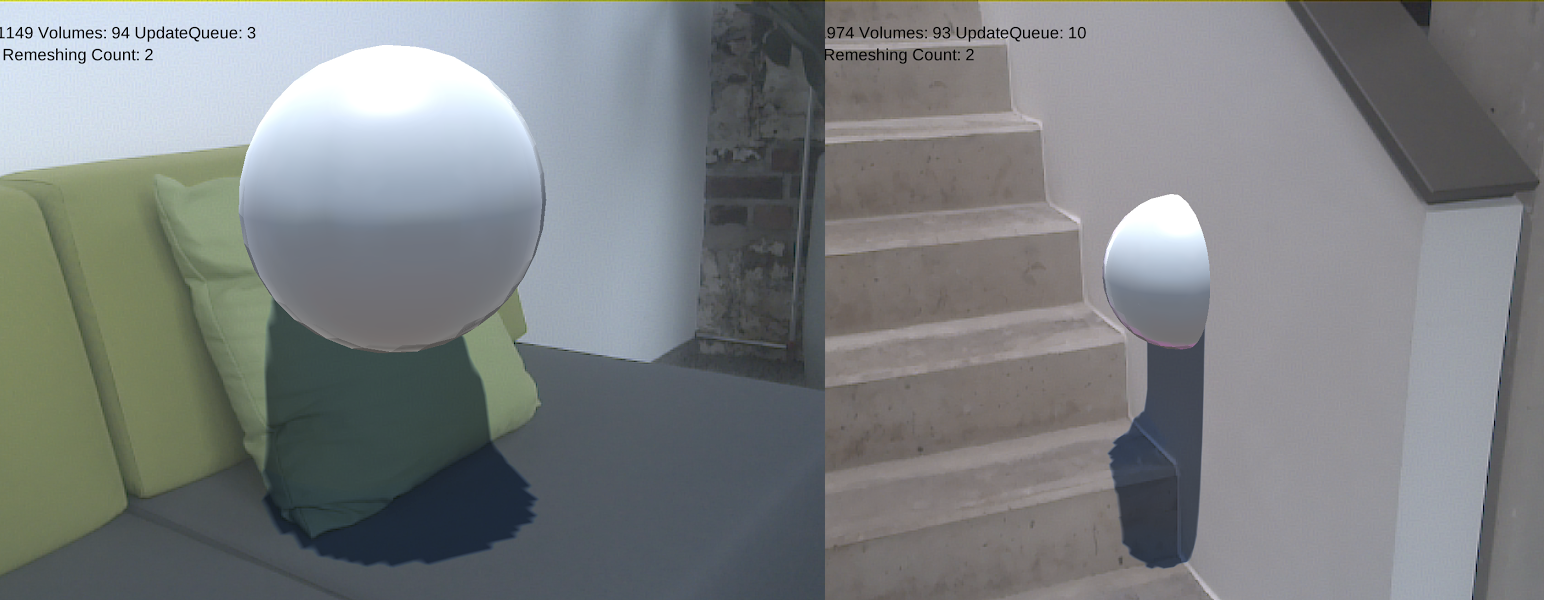
\includegraphics[width=1.0\textwidth]{content/images/shadow.png} 
  \caption{Unity Prototyp mit Schattenschlag auf den Polygonen der Chisel Rekonstruktion.}
  \label{fig:shadow}
\end{figure}

Ein weiterer Grund sich für ein Rekonstruktionsverfahren zu entscheiden, welches geometrische Primitiven der Szene generiert, ist die Möglichkeit, Interaktionen oder Schattenschlag mit den verfügbaren Techniken von OpenGL umzusetzen. Denn wenn ausschließlich die Tiefeninformationen wie bei der Pointcloud Projektion bekannt sind, müssen für beispielsweise den Schattenschlag die entsprechenden Normalen der Oberfläche pro Tiefenwert bestimmt werden. Bei den Rekonstruktionen werden die Normalen bereits im Verfahren bestimmt oder sind nachträglich über die Polygone einfach zu bestimmen. Hierzu wurde in dieser Arbeit ein weiterer Proof of Concept umgesetzt, der mit Hilfe einer Chisel Rekonstruktion und dem Shadowmapping der Unity Engine, die Projektion einer virtuellen Kugel mit Schattenschlag in einer realen Umgebung ermöglicht. Zwei Beispiele der Anwendung sind in Abbildung \ref{fig:shadow} zu sehen.


\section{Ausblick}

Im Laufe der Umsetzung und der Auswertung der Verfahren sind noch weitere Ideen entstanden, die nicht näher verfolgt werden konnten, aber durchaus eine Verbesserung der Qualität und Performance in den Verfahren beitragen könnten. Um die Qualität der Rekonstruktionen zu verbessern, könnte näher untersucht werden, wie sich das Filtern der Pointcloud vor der Integration in die Rekonstruktion auswirken könnte. Dazu kann die Pointcloud zunächst zu einem Tiefenbild projiziert werden und darauf hin mit dem Guided Filter oder dem \enquote{Guided Depth Upsampling} Verfahren von \citet{Ferstl_2013_ICCV} auf Basis des Farbbildes verbessert werden. Denn bis jetzt wurde erst immer nach der Rekonstruktion eine Optimierung der Tiefeninformationen vorgenommen. Hierdurch könnten Ungenauigkeiten und Ausreißer schon vor der Rekonstruktion reduziert werden. 

Wie zuvor erwähnt, können neben dem Guided Filter noch deutlich komplexere Verfahren eingesetzt werden, wie das \enquote{Guided Depth Upsampling} Verfahren von \citet{Ferstl_2013_ICCV}, die ein Tiefenbild auf Basis der Farbbilder optimiert. Da diese in der Regel jedoch komplexer als der Guided Filter sind, wäre ein Einsatz auf dieser mobilen Plattform nicht performant genug. Für den produktiven Einsatz des Guided Filters wäre generell eine eigene Implementation sinnvoll, um den OpenCV Anteil aus der prototypischen Umsetzung herausnehmen zu können. Das würde zunächst den Transformationsaufwand zu OpenCV von \(80 ms\) vermeiden. Außerdem wäre es denkbar den Guided Filter komplett im OpenGL Fragmentshader umzusetzen, wodurch eine parallele Verarbeitung der GPU diesen Prozess deutlich beschleunigen würde. 

Während der Implementierung und Recherche zu den verschiedenen Ansätzen zur Realisierung der AR Überdeckung mit Project Tango, wurden viele neue Schnittstellen in der Project Tango Bibliothek von Google veröffentlicht\footnote{Project Tango Release Notes - https://goo.gl/ueGBtn (21.03.16)}.  Unter Anderem wurde zuletzt zum Beispiel eine Methode für das Filtern des Tiefenbildes mit Hilfe des Farbbildes durch den Bilateral Filter veröffentlicht\footnote{Depth Interpolation Support Functions - https://goo.gl/kDdq21 (21.03.16)}. Nach den Recherchen zu den Filtern ist hier eigentlich der Guided Filter der leistungsfähige Ansatz. Außerdem wurde die interne Chisel Implementation für eine Rekonstruktion unter der Unity Engine veröffentlicht. Diese scheint speziell auf die Charakteristika der Tango Hardware abgestimmt zu sein, und liefert im beschriebenen Prototypen aus Abbildung \ref{fig:shadow} präzise Rekonstruktion mit einer Auflösung von \(5cm\).

Seitdem die Firma Lenovo eine Kooperation\footnote{Lenovo News - http://goo.gl/jFLNyn (21.03.16)} mit Google angekündigt hat, in der sie das erste Endverbraucher Gerät mit Project Tango Hardware und Software entwickeln werden, verspricht Project Tango eine einheitliche Technologie für das Motion Tracking, die Tiefenwahrnehmung und der Umgebungswiedererkennung auf mobilen Endgeräten zu werden. Auch Intel arbeitet mit Google zusammen\footnote{Intel\textregistered RealSense\textsuperscript{TM} Developer Kits - http://goo.gl/j4Y18A (21.03.16)} und ermöglicht in ihrer Konkurrenztechnologie RealSense\textsuperscript{TM} den Betrieb von Project Tango Anwendungen. 

* Holo Lense?
	
	